
  
Virtual reality is a technology which is often regarded as a natural extension to 3D computer graphics with advanced input and output devices \citep{Jayaram1997}. Ryan (2001) defined it as an “interactive, immersive experience generated by a computer” \citep{Ryan2001}. And according to G.C. Burdea and Coiffet (2017) “it is a generated computer graphics used to create a realistic-looking world that responds to the user’s input (gestures, verbal commands, etc.)” \citep{burdea2017virtual}. Virtual reality places the users inside the experience instead of viewing a screen in front of them, the users will be immersed inside a 3D world. As shown in Figure \ref{fig:3I} Three elements are needed to construct a virtual reality situation: immersion, interaction, and imagination. They are called the “3I’s” of virtual reality \citep{Hu2016}.


\begin{wrapfigure}{r}{0.30\textwidth} %this figure will be at the left
    \centering
    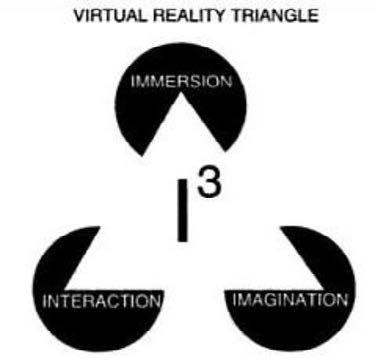
\includegraphics[width=0.30\textwidth]{3I}
    \caption{The 3I's of Virtual Reality - © 2003 by John Wiley \& Sons Inc. All rights
reserved}
    \label{fig:3I}
\end{wrapfigure}

1. \textbf{Immersion:} it is the virtual reality situation where the user feels personally inside the
scene and immerse inside the simulated virtual world.



2. \textbf{Interaction:} The interactive feedback between the user
and the virtual environment. Since it is a man-machine
interface, the system should promptly respond to the
user’s actions.


3. \textbf{Imagination:} The scene design and the construction of
the environment formulated with imagination for a
better user simulated experience.


  
  
  
The idea is to develop a new application to show Palestine with 360$^{\circ}$ videos, but it will include a part of one of the demolished villages before 1948. To rebuild one of those villages we need to know the structure of the village and how it looked like. The data about the structure of the village will be collected through personal stories, old pictures, British mandate aerial photos, and some maps made by a few people who lived in those villages. 
  
  
In the master project, a pre-study of the project will be conducted with Palestinians who live in the diaspora through interviews and workshops.  The Interview is a highly used method of collecting data in qualitative social research methods” \citep{Anyan2013}.  Kvale(1983)  described the purpose of as a method collection in social research as “... to gather descriptions of the life-world of the interviewee with respect to interpretation of the meaning of the described phenomena”  \citep{Kvale1983}. Semi-structured interviews will be used for collecting stories and exploring personal experiences about the Palestinians displacement and their relation with Palestine after living abroad. A questions guideline will be prepared for the interviews with  open-ended questions allowing a discussion with the interviewee rather than  formulated questions and answers.

After the interview some insights would be collected from the interviewee through a participatory design workshop. Participatory design (PD) is a set of theories, practices, and studies related to end-users as full participants in activities leading to software and hardware computer products and computer-based activities  \citep{Muller2003}. The field is extraordinarily diverse,  drawing on fields such as user-centered design, graphic design, software engineering, architecture, public policy, psychology, anthropology, sociology, labor studies, communication studies, and political science, and from localized experiences in diverse national and cultural contexts \citep{Gregory2003}.  Personal stories might give the ability for some refugees to draw the houses of their villages how they remember it. Applying a workshop for some of the Palestinian refugees to re-draw their houses would demonstrate a better image for the construction of the village, and that will give them the ability to tell us what they would like to see. houses, public places, walking paths between the houses, farms...etc. 
Information and communications technologies (ICT) artifacts should react to changing conditions of a social system \citep{Wulf2011}. Design case studies give us the ability to understand the relationship between social practice and the design of ICT artifacts that are built to support those practices, It is not so much about high tech, but about high-value \citep{Volker2013}. Design Case Studies ideally consist of three phases: (1) Analyze and particularly describe a social practice on a micro-level, as well describing the tools, media and their usage. (2) Describe the ICT artifacts from a product and from a process perspective, like the design concepts, and the applied design methods. (3) Document the introduction, appropriation and the potential re-design of the ICT artifact, documentation allows analyzing the trans-formative impact of certain functions and design options \citep{Volker2013}. Design case studies will allow us to check with the Palestinian refugees the tools or the practice that they do to see or to feel the connection with Palestine as a country and with their villages. After understanding their tools or practice, we can build a design depending on a specific design concept and methods. By letting them trying the prototype we will have general feedback about the interaction of the user with the App, and what would need to maintain and what kind of things needs to be re-designed. Design case studies will give us a general overview of the design concept and full fill us with the answers for the "how" and "why" about using the design methods.   
The Application will start by showing an overview of the whole map of historical Palestine. Points of interest will hover over the cities, the user will select a point of interest through the gaze feature. After selection, the map will be zoomed to the city location and will show more specified places within the city and the villages surrounding the city. The user will be transferred to a 360$^{\circ}$ video of the desired place, and inside the 360$^{\circ}$ video the user can commute inside the village for instance through the points of interest. sound of the surrounding environment will be added to the videos, as well as narrating the history and personal stories about the place. Within the demolished village, the user will have the ability to see how is the village look like now, and how it used to look like before 1948 by selecting an interactive button to travel in time. The user will have the ability to move back to the main map to choose to see different locations. All the methods that are used will help us to develop and collect the information and the data that is needed for the application and to be presented to the user.
\section{Related Work}
\section{Example projects}
\textbf{Auschwitz Virtual Tour}\footnote{Auschwitz VR Tour-\url{https://youtu.be/EOM_CxAKB_Y}}: The German broadcasting institution WDR made a 360o
documentary in Auschwitz concentration camp. Within the documentary, some Holocaust
survivors tell their stories. While listening to the stories and seeing the different locations in
the camp the user could feel the fear and horror that people suffered from. The video
immerses the user through the sound of the surrounding environment in the camp, you can
hear the wind and the sound gives a slight feeling of the cold weather over there. The
experience is immersive, but there is no interactivity with the user.


\textbf{Clouds over Sidra}\footnote{The Za’atari camp VR Tour-\url{https://youtu.be/mUosdCQsMkM}}: A 12 years old girls’ daily life story at the Za’atari refugee camp in Jordan
showed in virtual reality. The camp is a home for 80,000 Syrian refugees, half of them are
children(“Syrian Refugee Crisis – UN Virtual Reality,” 2015). The documentary was made by
the United Nation to raise awareness about the Syrian crisis. The video contained a number
of short videos from different parts of the camp, and it’s being synchronized while Sidra
narrates her story. It is more like watching a video with empathy than being immersed, but
the video presents the real life of the camp. Although the difference that while watching and
listening to the story, the user observes the people how they actually survive and live in the
camp. Therefore, the user does not have to imagine how is life over there.


\textbf{Carne y arena}\footnote{Carne y Arena Trailer-\url{https://youtu.be/zF-focK30WE}} : A highly professional
Virtual reality project that puts viewers
into the harsh life of an immigrant. The
user is placed among a group of
Mexican immigrants passing the
borders into the U.S. It was written and
directed by Alejandro G. Iñárritu. It Is a
full virtual reality experience; the user
needs to reserve an individual session
on the website. According to Pinotti (2017) you go in a dark room; your feet are on the sand (coarse grain, rough feeling) then, two assistants welcome you and provide you with the
necessary devices: an Oculus Rift headset, a backpack connected via cables to a powerful
computer and you are ready to be caught up in a nightmare \citep{Pinotti2017}. The project is
subtitled by ‘Virtually present, Physically invisible’. Pinotti (2017) defined, Virtually present:
“you are transported in the middle of the desert, among men, women, and children who try
their voyage of hope”. Physically invisible: “you are present, but nobody sees you and after a
while, you start to feel the need to be noticed and seek acknowledgment of social
recognition” \citep{Pinotti2017}. The project was developed with high technology, like 3D
modeling, visual effects, sound. The interaction of the user and the feeling of “being there”
by placing the user in a special environment, leads to a unique experience of immersion.

